\chapter{Conclusion} % Main chapter title

\label{Chapter:Conclusion}

The complexities involved in the development of sustainable cities cannot be overlooked by researchers and policy makers. The concept of sustainability has over the years been over-simplified. This has led to researchers and policy makers focusing mostly on the multi-functional dimensions of sustainability to the neglect of the complementary and conflicting roles of these functions. This study, which seeks to determine the nexus between urban agriculture and sustainable cities has helped in clarifying the various divergent arguments in the sustainable city discourse. Conceptually, this research relied on a framework that assesses the sustainability of cities from the economic, social and environmental sustainability dimensions. Its strengths lie in the use of a comprehensive set of indicators to measure sustainable cities, which makes the framework relevant to both research and policy making.

The results show that the social, economic and environmental functions of urban agriculture have both positive and negative outcomes. The review further showed that, the benefits of urban agriculture especially the ecological and social dimensions have been grossly underestimated. This has led researchers such as Veenhuizen (2006) and Yamusa (2014) to argue that the contributions of urban agriculture to sustainable cities have been exaggerated. However, the review indicates that urban agriculture can propel the drive of many countries, especially in the Global South, towards sustainable development. Varying contextual factors such as climate, topography, increasing rate of urbanisation, land commodification and scarcity affect the nature of agricultural activities. For instance, vertical farming techniques and container gardens may be appropriate in compact cities where land scarcity is highly prevalent. Similarly, water-efficient technologies and wastewater reuse should be encouraged in cities within the arid and semi-arid regions of the world.

In cities with relatively large vacant lands, urban agriculture should be sustained through conscious integration into city land use planning and zoning processes. In the developed countries where there is effective enforcement of land use regulations, ecologically-sensitive areas can be protected through zoning regulations and can provide spaces for urban farming practices that reinforce their ecological functions. However, in developing countries such as Ghana where there is ineffective enforcement of land use regulations, urban agriculture could play an important role in helping to protect these ecologically sensitive areas. Ecologically sensitive areas such as wetlands play very significant functions in the city such as flood management. We therefore suggest that zoning these areas which are already in use for urban agriculture could serve a dual function of protecting them as well as sustaining urban agriculture. Emphasis is on responsible agriculture, which will largely protect the ecological functions of these land uses. Urban green spaces and ecologically-sensitive areas that will be zoned for agricultural purposes must be acquired by the government and city authorities by paying the right amount of compensations to the land owners. This will help to address the problem of land commodification by traditional authorities and other land owners.

The general conclusion is that the nature of agriculture in the cities should be informed by the unique characteristics of that city. Agriculture should be sustained in the landscape of these cities due to its profound roles in the sustainable-city discourse.

%\begin{figure}[th]
%\centering
%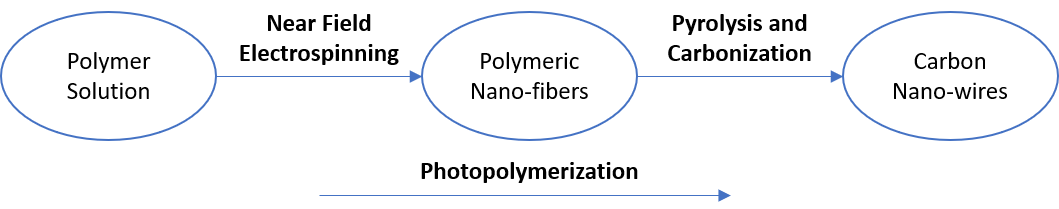
\includegraphics[width=0.95\textwidth]{./Figures/FabricationProcess.png}
%\decoRule
%\caption[Carbon Nano-wires Fabrication Process]{Fabrication process of carbon nano-wires to achieve through the proposed dissertation.}
%\label{fig:fabricationFlowChart}
%\end{figure}

%\begin{equation}
%\left(\tau _t^e-\frac{\tau _n^e \text{dr}}{\text{dz}}\right) 2 \pi  r+\frac{d \left(\pi  r^2
%   \left(\tau _{\text{zz}}-p\right)\right)}{\text{dz}}+\frac{\gamma  \text{dr} 2 \pi  r}{r
%   \text{dz}}+\rho  g \pi  r^2=\frac{d \left(\rho  \pi  r^2 v^2\right)}{\text{dz}}
%\label{eq:linearMomentum}
%\end{equation}